\documentclass[12pt]{amsart}
\usepackage{fullpage}
\makeatletter

%% AMS
\usepackage{amsmath,amssymb,latexsym}

%% Theorems
\usepackage{xcolor}
\definecolor{darkgreen}{rgb}{0,0.45,0} 
\usepackage[pagebackref,colorlinks,citecolor=darkgreen,linkcolor=darkgreen]{hyperref}
\usepackage{cleveref,aliascnt}
\usepackage{amsthm}
\def\defthm#1#2#3{%
  %% Ensure all theorem types are numbered with the same counter
  \newaliascnt{#1}{thm}
  \newtheorem{#1}[#1]{#2}
  \aliascntresetthe{#1}
  %% Tell cleveref's \cref what to call things
  \crefname{#1}{#2}{#3}}
\newtheorem{thm}{Theorem}[section]
\crefname{thm}{Theorem}{Theorems}
\theoremstyle{definition}
\defthm{defn}{Definition}{Definitions}
%\theoremstyle{remark}
\defthm{rmk}{Remark}{Remarks}
\defthm{advrmk}{Advanced Remark}{Advanced Remarks}
\newenvironment{adv}{\small\begin{advrmk}}{\end{advrmk}}
\defthm{eg}{Example}{Examples}
\defthm{egs}{Examples}{Examples}
\defthm{sage}{Sage}{Sages}

%% Reference format for sections
\crefformat{section}{\S#2#1#3}
\Crefformat{section}{Section~#2#1#3}
\crefrangeformat{section}{\S\S#3#1#4--#5#2#6}
\Crefrangeformat{section}{Sections~#3#1#4--#5#2#6}
\crefmultiformat{section}{\S\S#2#1#3}{ and~#2#1#3}{, #2#1#3}{ and~#2#1#3}
\Crefmultiformat{section}{Sections~#2#1#3}{ and~#2#1#3}{, #2#1#3}{ and~#2#1#3}
\crefrangemultiformat{section}{\S\S#3#1#4--#5#2#6}{ and~#3#1#4--#5#2#6}{, #3#1#4--#5#2#6}{ and~#3#1#4--#5#2#6}
\Crefrangemultiformat{section}{Sections~#3#1#4--#5#2#6}{ and~#3#1#4--#5#2#6}{, #3#1#4--#5#2#6}{ and~#3#1#4--#5#2#6}

%% Use the theorem counter for equations as well
\let\c@equation\c@thm
\numberwithin{equation}{section}

%% Pictures
\usepackage{tikz}
\usepackage{graphicx}

%% Differentials
\newcommand{\dd}{\ensuremath{\mathrm{d}}}
\newcommand{\ed}{\ensuremath{\mathrm{d}\wedge}}

%% Differentials of variables
\newcommand{\dx}{{\ensuremath{\dd x}}}
\newcommand{\dy}{{\ensuremath{\dd y}}}
\newcommand{\dz}{{\ensuremath{\dd z}}}
\newcommand{\dzbar}{{\ensuremath{\dd \bar{z}}}}
\newcommand{\dt}{{\ensuremath{\dd t}}}
\newcommand{\du}{{\ensuremath{\dd u}}}
\newcommand{\dv}{{\ensuremath{\dd v}}}
\newcommand{\df}{{\ensuremath{\dd f}}}
\newcommand{\dg}{{\ensuremath{\dd g}}}
\renewcommand{\dh}{{\ensuremath{\dd h}}}
\newcommand{\dr}{{\ensuremath{\dd r}}}
\newcommand{\drho}{{\ensuremath{\dd \rho}}}
\newcommand{\dtheta}{{\ensuremath{\dd \theta}}}
\newcommand{\dphi}{{\ensuremath{\dd \phi}}}
\newcommand{\dpx}{{\ensuremath{\dd \pt{x}}}}

%% Not differentials of anything
\usepackage[T1]{fontenc}
\usepackage{lmodern}
\newcommand{\dl}{\ensuremath{\mathrm{\dj}\ell}}
\newcommand{\dA}{\ensuremath{\mathrm{\dj}A}}
\newcommand{\dV}{\ensuremath{\mathrm{\dj}V}}
\newcommand{\dn}{\ensuremath{\mathrm{\dj}\vc{n}}}

%% Wedge product
%\newcommand{\wedge}{\wedge}

%% Partial derivatives
% \newcommand{\pder}[2]{\frac{\partial #1}{\partial #2}}
% \newcommand{\pdertwo}[2]{\frac{\partial^2 #1}{\partial #2^2}}
% \newcommand{\pdermixed}[3]{\frac{\partial^2 #1}{\partial #2 \,\partial #3}}
\newcommand{\pder}[2]{{#1}_{#2}}
\newcommand{\pdertwo}[2]{{#1}_{{#2}{#2}}}
\newcommand{\pdermixed}[3]{{#1}_{{#2}{#3}}}

%% Transposing vectors into forms
\newcommand{\tr}[1]{{#1}^\top}
\newcommand{\ptr}[1]{{(#1)}^\top}

%% Hodge star on forms
\newcommand{\str}[1]{{#1}^*}
\newcommand{\pstr}[1]{{(#1)}^*}

%% Points and vectors
\newcommand{\pt}[1]{\mathbf{#1}}
\newcommand{\ptc}[1]{(#1)}
\newcommand{\ptx}{\pt{x}}
% \newcommand{\vc}[1]{\vec{#1}}
\newcommand{\vc}[1]{\mathbf{#1}}
\newcommand{\vcc}[1]{(#1)}
\newcommand{\lrvcc}[1]{\left(#1\right)}

%% Vector operations
\newcommand{\mgn}[1]{\Vert #1 \Vert}
%\newcommand{\dotp}[2]{\langle #1 , #2 \rangle}
\newcommand{\dotp}[2]{#1 \cdot #2}
\newcommand{\crossp}[2]{#1 \times #2}

%% Vector calculus operations
\newcommand{\grad}[1]{\nabla #1}
\renewcommand{\div}[1]{\nabla \cdot #1}
\newcommand{\curl}[1]{\nabla \times #1}

%% Fractions
\newcommand{\half}{\ensuremath{\textstyle\frac{1}{2}}}
\newcommand{\halfi}{\ensuremath{\textstyle\frac{1}{2i}}}
\newcommand{\halfpii}{\ensuremath{\textstyle\frac{1}{2\pi i}}}
\newcommand{\third}{\ensuremath{\textstyle\frac{1}{3}}}

%% Orders
\renewcommand{\th}{^{\mathrm{th}}}
\newcommand{\st}{^{\mathrm{st}}}

%% Approximation to specified order
\newcommand{\apx}[1]{\mathrel{\overset{#1}{\approx}}}

%% Riemann sums
\newcommand{\rstag}[2]{{#1}_{#2}^*}

%% Complex conjugation
\newcommand{\conj}[1]{\bar{#1}}
\newcommand{\zbar}{\conj{z}}
\newcommand{\wbar}{\conj{w}}

%% Parametrized curves
\newcommand{\curve}{C}
\newcommand{\curvept}{\mathbf{x}}
\newcommand{\dcurvept}{\dd\mathbf{x}}
\newcommand{\curvex}{x}
\newcommand{\curvey}{y}
\newcommand{\curvez}{z}

%% Regions
\newcommand{\region}{R}
\newcommand{\bdry}{\partial}

%% Parametrized surfaces
\newcommand{\surf}{S}
\newcommand{\surfx}{x}
\newcommand{\surfy}{y}
\newcommand{\surfz}{z}

%% Integrals of differential forms.  The only argument is the
%% integration manifold; the differential form just comes afterwards.
\newcommand{\lint}[1]{\int_{#1}} % line integral over a curve
\newcommand{\sint}[1]{\iint_{#1}} % surface integral form over a surface
\newcommand{\vint}[1]{\iiint_{#1}} % volume integral over a spatial region

%% "Classical" integrals.  For these the integrand is a *function*
%% (well, technically, an expression with free variables) which is
%% given as a second argument.
\newcommand{\dint}[2]{\iint_{#1} #2 \,\dA} % double integral over a plane region
\newcommand{\tint}[2]{\iiint_{#1} #2 \,\dV} % triple integral over a spatial region
\newcommand{\itint}[4]{\int_{#2}^{#3} #4 \,\dd #1} % ordinary one-variable integral over an interval
\newcommand{\itdint}[7]{\int_{#2}^{#3} \int_{#5}^{#6} #7 \,\dd #4\,\dd #1} % double iterated integral
% Can't have more than 9 parameters
%\newcommand{\ittint}[10]{\int_{#2}^{#3} \int_{#5}^{#6} \int_{#8}^{#9} #10 \,\dd #7\,\dd #4\,\dd #1} % triple iterated integral
\makeatletter
\newcommand{\ittint}[3]{\int_{#2}^{#3} \@ittint #1}
\newcommand{\@ittint}[8]{\int_{#3}^{#4} \int_{#6}^{#7} #8 \,\dd #5\,\dd #2\,\dd #1} % triple iterated integral
\makeatother

%% Textbooks
\usepackage{version}
\includeversion{notextbook}
\excludeversion{stewart}
\excludeversion{hugheshallett}
\excludeversion{rogawski}

\makeatother

\title{On differential forms}
\begin{document}
\maketitle

In your previous calculus classes, you may or may not have encountered \emph{differential forms} by name.
However, you've certainly met them, even if you didn't realize it.
When you write
\[ \int_{x=a}^b f(x) \,\dx \]
the thing being integrated, ``$f(x) \,\dx$'', is a differential form.

You may have been told that the ``$\dx$'' is simply a notation that indicates which variable we're integrating, but this is a lie.
In multivariable calculus, we can no longer maintain this fiction: we have to treat differential forms as honest objects.
Fortunately, we also have two advantages over one-variable calculus in understanding differential forms.
Firstly, we have \emph{vectors} at our disposal; and secondly, some things are actually \emph{less} confusing in \emph{more} dimensions, because there are fewer coincidences to get confused by.
(Unfortunately, in three dimensions --- which is of course the most common and the most useful number, since it is the dimension of the space we live in --- there is still one very confusing coincidence remaining.
This comes from the fact that $1+1=3-1$, and is the reason that the \emph{cross product} of vectors exists.
We will come back to this later.)

\section{Differential forms}
\label{sec:differential-forms}

If $\dx$ isn't just a notation indicating the integration variable, what is it?
If you encountered differentials in one-variable calculus, you may have been told that $\dx$ is a small change in $x$ (sometimes denoted $\Delta x$), or even an ``infinitesimal'' change in $x$.
These are not wrong, but with vectors we can give a better definition.

\begin{defn}
  A \textbf{differential form} is a function whose input is a point $\ptx$ \emph{and} a vector based at $\ptx$.
  We denote the vector by $\dpx$.
\end{defn}

In $n$ dimensions, the point $\ptx$ has $n$ coordinates, as does the vector $\dpx$.
As usual, in 2 or 3 dimensions we denote the coordinates of $\ptx$ by $\ptc{x,y}$ or $\ptc{x,y,z}$.
Similarly, we denote the coordinates of $\dpx$ by $\vcc{\dx,\dy}$ or $\vcc{\dx,\dy,\dz}$.
We can then describe a differential form by a formula involving these coordinates $x,y,z,\dx,\dy,\dz$.

We usually denote differential forms by lowercase Greek letters such as the following.
\begin{itemize}
\item $\omega$ (omega, not to be confused with the English letter $w$)
\item $\eta$ (eta, not to be confused with the English letter $n$)
\end{itemize}
Since a differential form $\omega$ is a function of a point and a vector, we would write $\omega(\ptx,\dpx)$ for the value of $\omega$ at a point $\ptx$ and a vector $\dpx$, or $\omega(x,y,\dx,\dy)$ if we want to emphasize all the coordinates.

\begin{egs}\label{egs:differential-forms}
  The following are all differential forms:
  \begin{gather*}
    x^2 \,\dx + 2xy \, \dy\\
    \half({x-z}) \,\dx - 4\, \dy + e^y \,\dz\\
    1 + \dx + \half \dx^2 + \third \dx^3\\
    \sin(x + \dx) - \sin(x)\\
    \sqrt{\dx^2+\dy^2}
  \end{gather*}
\end{egs}

Note that although $\dx$ is two letters, we regard it as one symbol standing for one variable.
In particular, an expression such as $\dx^2$ means $(\dx)^2$, not $\dd(x^2)$.
(We will give a different meaning to $\dd(x^2)$ in \cref{sec:differentials}.)

The first two of \cref{egs:differential-forms} are special in the following way.

\begin{defn}
  A \textbf{linear} differential form is one defined by an expression such as
  \[ f(\ptx) \, \dx + g(\ptx) \, \dy + h(\ptx) \, \dz. \]
  Here $f$, $g$, and $h$ are functions of the point $\ptx$ only, and each of them is multiplied by one of the coordinates of $\dpx$.
\end{defn}

Most mathematicians only use the term ``differential form'' for linear ones.
However, the more general ones are quite useful.

\begin{adv}
  To be more precise, the differential forms we are considering so far are \emph{1-cojet differential 1-forms}.
  Later on, we will encounter both $k$-cojet differential forms and differential $n$-forms for larger values of $k$ and $n$.
  However, until then, we will just use ``differential form'' for the notion defined above.
\end{adv}

It is appropriate to think of $\dpx$ as a \emph{small change} in the point $\ptx$, so that its coordinates such as $\dx$ and $\dy$ are small changes in the values of the coordinates $x$ and $y$.
Specifically, we can think of $\dpx$ as the vector \emph{from} the point $\ptx$ \emph{to} a slightly shifted point, $\ptx+\dpx$.
\begin{center}
  \begin{tikzpicture}[scale=1.6]
    \draw[<->] (-1,0) -- (3,0);
    \draw[<->] (0,-1) -- (0,3);
    \node[circle,fill,purple,label={[purple]$\ptx$}] (x) at (1.5,2) {};
    \node[circle,fill,purple,label={[purple]right:$\ptx+\dpx$}] (x2) at (2,1.5) {};
    \draw[very thick,purple,->] (0,0) -- (x);
    \draw[very thick,blue,->] (x) -- node[auto] {$\dpx$} (x2);
  \end{tikzpicture}
\end{center}
Nothing in the definition forces $\dpx$ to be ``small'', but generally we are only interested in the values of a differential form when $\dpx$ is small.
Specifically, by \emph{small} we mean \emph{small relative to the values generally taken by $x$}.
For instance, if $x=3$, then a possible small change would be $\dx = 0.01$.
In this case, a differential form such as $\dx^2$ is an \emph{even smaller} change, since $\dx^2 = 0.0001$.

We say that $\dx$ is a \emph{first order} form while $\dx^2$ is \emph{second order}.
Similarly, we say that $x$ itself is \emph{zeroth order}, as is any function value $f(\ptx)$ not involving $\dpx$.

Every linear form is first-order: when we multiply a zeroth order form like $f(\ptx)$ by a first order one like $\dx$, the result is first order.
For instance, if $f(x) = 4$ and $\dx = 0.001$, then $f(x)\,\dx = 0.004$, which is about the same size as $\dx$.

The concept of order can be applied even to forms that are not polynomials in $\dx$.
For instance, if $\dx=0.01$, then $\sin(\dx) \approx 0.0099998$, which is about the same size as $\dx$.
Thus, it is reasonable to say that $\sin(\dx)$ is also first-order.
On the other hand, still with $\dx=0.01$, we have $\cos(\dx) - 1 \approx -0.00005$, which is much smaller than $\dx$ and about the same size as $\dx^2$.
Thus, it is reasonable to say that $\cos(\dx) - 1$ is second-order.

We will not make precise the general notion of ``order''; it can be done, but it is a bit complicated and not necessary for our purposes.
(If you're curious, see the optional handout.)
All that we will need is a definition of when a differential form is \emph{smaller than first order} (e.g.\ second-order or third-order).
This is because in calculus, we are concerned with \emph{approximations to first order}, also known as \emph{linear approximations}; and forms that are smaller than first order do not affect these approximations.
Thus, we will call them \emph{negligible} (to first order).

\begin{defn}\label{def:negligible}
  A differential form $\omega$ is called \textbf{negligible} at a point $\ptx$ if
  \[ \lim_{\dpx\to\vc{0}} \frac{\omega(\ptx,\dpx)}{\mgn{\dpx}} = 0. \]
\end{defn}

Recall that definitions in mathematics introduce a \emph{new} meaning for a word.
Thus, \emph{from now on} (in this class) the word ``negligible'' \emph{will mean} what this definition says it does.
Our previous discussion was only motivational; the definition is the ``gold standard'' for the meaning of the word.

Note also that the limit in \cref{def:negligible} is a \emph{vector} limit.
In two or three dimensions, we could write it equivalently as
\[ \lim_{(\dx,\dy)\to(0,0)} \frac{\omega(x,y,\dx,\dy)}{\sqrt{\dx^2+\dy^2}} \qquad\text{or}\qquad
\lim_{(\dx,\dy,\dz)\to(0,0,0)} \frac{\omega(x,y,z,\dx,\dy,dz)}{\sqrt{\dx^2+\dy^2+\dz^2}}
\]
respectively.
Recall that this means that we allow $\dpx$ to approach $\vc{0}$ ``in all possible ways''.
\begin{notextbook}Two- and three-dimensional limits should be discussed in your textbook.\end{notextbook}%
\begin{stewart}Two- and three-dimensional limits are discussed in section 11.2 of the textbook.\end{stewart}

The first thing to do in understanding a definition is to look at some examples.
If we chose the definition well, the examples will justify our motivation.

\begin{eg}
  The differential form $\dx^2$ is negligible at any point.
  To see this, note that
  \[ \frac{\dx^2}{\mgn{\dpx}} = \frac{\dx}{\mgn{\dpx}} \,\dx \]
  and $\frac{\dx}{\mgn{\dpx}}\le 1$ everywhere, while $\lim_{\dpx\to\vc{0}} \dx = 0$.
  Thus, the limit of their product is also $0$.
  Similarly, the following differential forms are all negligible:
  \[ \dy^2 \qquad \dx\,\dy \qquad \dx^3 \qquad \dx\,\dy^2\,\dz \]
\end{eg}

\begin{eg}
  By a similar argument, if $\omega$ is bounded for values of $\dpx$ near $\vc{0}$, while $\eta$ is negligible at $\ptx$, then their product $\omega\eta$ is also negligible at $\ptx$.
  In particular, this is true if $\omega$ is a function of $\ptx$ only, at any point where it is defined.
  For instance, the following differential forms are negligible:
  \begin{gather*}
    x^2\,\dx\,\dy\\
    e^{-x^2+y^2} \,\dy^2
  \end{gather*}
\end{eg}

\begin{eg}
  If $\omega$ and $\eta$ are negligible at $\ptx$, then so is their sum $\omega+\eta$, by the sum rule for limits.
  Thus, the following differential forms are negligible:
  \begin{gather*}
    \dx^2 + \dy^2\\
    x^2 \,\dx\,\dy + e^{y}\,\dy\,\dz^2
  \end{gather*}
\end{eg}

Notice that all the examples of negligible forms are what we would intuitively call second-order or higher.
We will continue to use the informal terminology of ``first-order'', ``second-order'', and so on when discussing forms.
However, in definitions and theorems we will use only the term ``negligible'' that we have defined precisely.


\section{Graphing differential forms}
\label{sec:graphing-differential-forms}

A differential form should be thought of as giving for each point $\ptx$, a function of the vector $\dpx$, which represents the ``displacement from $\ptx$'' of another point (namely, the point $\ptx+\dpx$).
In addition, we generally only care about this function for small values of $\dpx$.

Our first idea about how to graph such a thing might be to draw at each point $\ptx$ the graph of the corresponding function of $\dpx$, with its origin placed at $\ptx$.
However, there would be far too many of these graphs, and they would overlap so much as to make it impossible to see anything.
Instead we choose some representative (usually regularly spaced) values of $\ptx$ at which to draw graphs, and at each such point we draw only a small fragment of the graph of the corresponding function of $\dpx$.

This is easiest to do in one dimension.
For instance, we might graph the form $x\,\dx$ as follows.
\begin{center}
  \begin{tikzpicture}
    \draw[<->] (-5,0) -- (5,0);
    \draw[<->] (0,-2) -- (0,2);
    \draw (2,.2) -- (2,-.2) node[below right] {$1$};
    \draw (4,.2) -- (4,-.2) node[below right] {$2$};
    \draw (-2,.2) -- (-2,-.2) node[below] {$-1$};
    \draw (-4,.2) -- (-4,-.2) node[below left] {$-2$};
    \begin{scope}[blue,very thick]
      \draw (-.3,0) -- (.3,0);
      \draw (.7,-.15) -- (1.3,.15);
      \draw (1.7,-.3) -- (2.3,.3);
      \draw (2.7,-.45) -- (3.3,.45);
      \draw (3.7,-.6) -- (4.3,.6);
      \draw (-.7,-.15) -- (-1.3,.15);
      \draw (-1.7,-.3) -- (-2.3,.3);
      \draw (-2.7,-.45) -- (-3.3,.45);
      \draw (-3.7,-.6) -- (-4.3,.6);
    \end{scope}
  \end{tikzpicture}
\end{center}
Here at the point $(1,0)$ we have graphed a piece of the function $f(\dx) = 1\,\dx$, with its origin at $(1,0)$.
Similarly, at $(2,0)$ we have graphed a piece of $f(\dx) = 2\,\dx$, with its origin at $(2,0)$, and so on.

There is of course a lot of omitted information; we have not shown anything about the behavior of our differential form when $x$ is not one of the chose points.
Graphs of functions \emph{always} omit lots of information --- infinitely much information, in fact, corresponding to the behavior of the function outside the small window that we have chosen to display, as well as any behavior that is too small to see at our chosen scale.
(This is one of the dangers of relying too much on graphing calculators and computer algebra systems,
\begin{notextbook}as you may remember.\end{notextbook}%
\begin{stewart}as discussed in sections 1.4 and 4.4 of the textbook.\end{stewart})
Similarly, to graph a differential form usefully, we must not only choose an appropriate ``viewing rectangle'' but also choose at which values of $x$ to show a small graph fragment at.
For instance, when graphing the form $x\,\dx$, we could choose to show more small graph fragments, as follows:
\begin{center}
  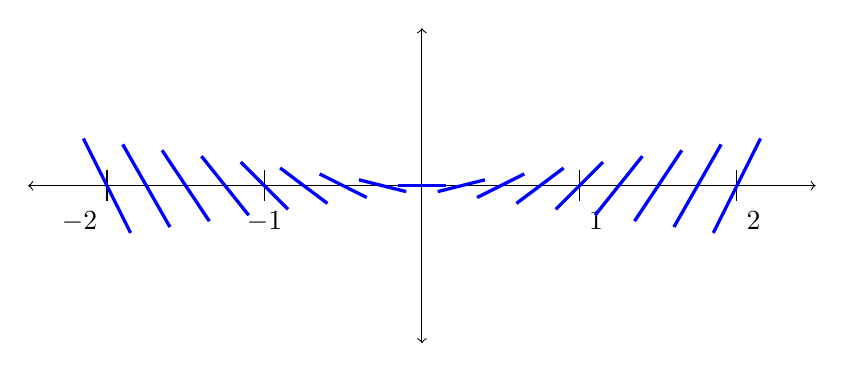
\begin{tikzpicture}
    \draw[<->] (-5,0) -- (5,0);
    \draw[<->] (0,-2) -- (0,2);
    \draw (2,.2) -- (2,-.2) node[below right] {$1$};
    \draw (4,.2) -- (4,-.2) node[below right] {$2$};
    \draw (-2,.2) -- (-2,-.2) node[below] {$-1$};
    \draw (-4,.2) -- (-4,-.2) node[below left] {$-2$};
    \begin{scope}[blue,very thick]
      \draw (-.3,0) -- (.3,0);
      \draw (.2,-.075) -- (.8,.075);
      \draw (.7,-.15) -- (1.3,.15);
      \draw (1.2,-.225) -- (1.8,.225);
      \draw (1.7,-.3) -- (2.3,.3);
      \draw (2.2,-.375) -- (2.8,.375);
      \draw (2.7,-.45) -- (3.3,.45);
      \draw (3.2,-.525) -- (3.8,.525);
      \draw (3.7,-.6) -- (4.3,.6);
      \draw (-.2,-.075) -- (-.8,.075);
      \draw (-.7,-.15) -- (-1.3,.15);
      \draw (-1.2,-.225) -- (-1.8,.225);
      \draw (-1.7,-.3) -- (-2.3,.3);
      \draw (-2.2,-.375) -- (-2.8,.375);
      \draw (-2.7,-.45) -- (-3.3,.45);
      \draw (-3.2,-.525) -- (-3.8,.525);
      \draw (-3.7,-.6) -- (-4.3,.6);
    \end{scope}
  \end{tikzpicture}
\end{center}
This gives an even better picture of the differential form, but of course it is more work to draw.
For the example $x\,\dx$, because the graphs change smoothly ``without any surprises'' in between the chosen values of $x$, there is not much lost by using fewer such points.
The important thing when drawing a graph is to convey all the ``important'' information about the behavior of the object being graphed.

Analogously, we would graph $x\,\dx^2$ as follows, drawing $f(\dx) = \dx^2$ with origin at $(1,0)$, and $f(\dx)=2\,\dx^2$ with origin at $(2,0)$, etc.
\begin{center}
  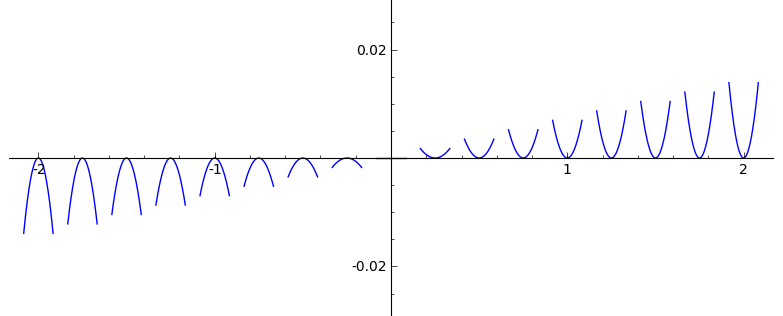
\includegraphics[width=0.8\textwidth]{x-dx2.png}
  % \begin{tikzpicture}
  %   \draw[<->] (-5,0) -- (5,0);
  %   \draw[<->] (0,-2) -- (0,2);
  %   \draw (2,.2) -- (2,-.2) node[below right] {$1$};
  %   \draw (4,.2) -- (4,-.2) node[below right] {$2$};
  %   \draw (-2,-.2) -- (-2,.2) node[above] {$-1$};
  %   \draw (-4,-.2) -- (-4,.2) node[above] {$-2$};
  %   \begin{scope}[blue,very thick]
  %     \draw (-.3,0) -- (.3,0);
  %     % \draw (.7,-.15) -- (1.3,.15);
  %     \draw (1.7,.3) to[out=-60,in=180] (2,0) to[out=0,in=-120] (2.3,.3);
  %     % \draw (2.7,-.45) -- (3.3,.45);
  %     \draw (3.7,.6) to[out=-75,in=180,looseness=.5] (4,0) to[out=0,in=-105,looseness=.5] (4.3,.6);
  %     % \draw (-.7,-.15) -- (-1.3,.15);
  %     \draw (-1.7,-.3) to[out=120,in=0] (-2,0) to[out=180,in=60] (-2.3,-.3);
  %     % \draw (-2.7,-.45) -- (-3.3,.45);
  %     \draw (-3.7,-.6) to[out=105,in=0,looseness=.5] (-4,0) to[out=180,in=75,looseness=.5] (-4.3,-.6);
  %   \end{scope}
  % \end{tikzpicture}
\end{center}
In the previous two examples, all the small graphs lay along the $x$-axis, because the differential forms being graphed had no zeroth order term.
If there is a zeroth order term, then the small graphs will lie along the graph of that term.
For instance, here is a graph of $-x^2 + 3\sin(x)\,\dx$, with the curve $y=-x^2$ shown as a dotted line for comparison:
\begin{center}
  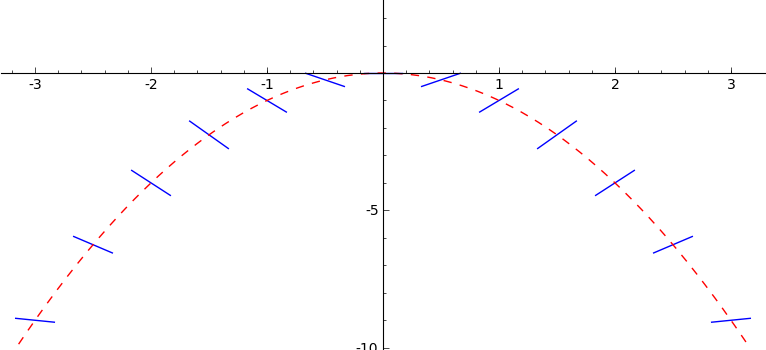
\includegraphics[width=0.8\textwidth]{mx2p3sinxdx.png}
  % \begin{tikzpicture}
  %   \draw[<->] (-5,0) -- (5,0);
  %   \draw[<->] (0,-5) -- (0,1);
  %   \draw (2,-.2) -- (2,.2) node[above] {$\frac\pi2$};
  %   \draw (4,-.2) -- (4,.2) node[above] {$\pi$};
  %   \draw (-2,-.2) -- (-2,.2) node[above] {$-\frac\pi2$};
  %   \draw (-4,-.2) -- (-4,.2) node[above] {$-\pi$};
  %   \draw (.2,-1) -- (-.2,-1) node[left] {$-\frac{\pi^2}{4}$};
  %   \draw (.2,-4) -- (-.2,-4) node[left] {$-\pi^2$};
  %   \begin{scope}[blue,very thick]
  %     \draw (-.3,0) -- (.3,0);
  %     \draw (.7,-.4) -- (1.3,-.1);
  %     \draw (1.7,-1.3) -- (2.3,-.7);
  %     \draw (2.7,-2.65) -- (3.3,-2.35);
  %     \draw (3.7,-4) -- (4.3,-4);
  %     \draw (-.7,-.4) -- (-1.3,-.1);
  %     \draw (-1.7,-1.3) -- (-2.3,-.7);
  %     \draw (-2.7,-2.65) -- (-3.3,-2.35);
  %     \draw (-3.7,-4) -- (-4.3,-4);
  %   \end{scope}
  %   \draw[purple,dashed] (-4,-4) to[out=60,in=120,looseness=1.97] (4,-4);
  % \end{tikzpicture}
\end{center}

\begin{sage}
  Sage doesn't know how to graph differential forms natively, but here is a short little function which teaches it how.
  You don't have to understand what it's doing; just copy the following lines into any Sage notebook and execute them.
\begin{verbatim}
def plotform(om,xmin,xmax,d,s):
    return sum([plot(om(x/d,dx-x/d),(dx,x/d-1/3/d,x/d+1/3/d),ymin=-s,ymax=s)
                for x in xrange(xmin*d,xmax*d+1)])
\end{verbatim}

  Now you can graph differential forms with the \texttt{plotform} function.
  The first argument is the differential form, the second and third are the minimum and maximum $x$ values, the fourth is the density of small graphs to draw (specifically, how many of them per unit $x$), and the fifth is the maximum $y$ value.
  The only wrinkle is that you have to tell Sage explicitly which variables in the differential form are which, by defining it first as a function rather than just passing it to \texttt{plotform} as an expression.
  For instance, here are the commands I used to generate the above graph of $x\,\dx^2$.
\begin{verbatim}
omega(x,dx) = x*dx^2
plotform(omega,-2,2,4,.05)
\end{verbatim}

  Remember that to graph more than one function on the same axes, you can just ``add'' them together with $+$.
  For instance, here is the command that I used to generate the above graph of $-x^2 + 3\sin(x)\,\dx$ with $y=-x^2$ shown for comparison:
\begin{verbatim}
omega(x,dx) = -x^2+3*sin(x)*dx
plotform(omega,-pi,pi,2,pi^2)+plot(-x^2,(x,-pi,pi),color='red',linestyle='dashed')
\end{verbatim}
\end{sage}

We now consider the graphs of some differential forms of particular interest associated to a function $f$ of $x$.
As a running example we will consider the following function:
\def\axes{
    \draw[<->] (-5,0) -- (5,0);
    \draw[<->] (0,-2) -- (0,2);
    \foreach \x in {1,2,3,4} \draw (\x,.2) -- (\x,-.2);
    \foreach \x in {1,2,3,4} \draw (-\x,.2) -- (-\x,-.2);
}
\def\fctn#1{\draw[#1] (-5,.3) to[out=30,in=170] (-4,1) to[out=-10,in=110] (-2,-1.2) to[out=-70,in=-130] (1,.2) to[out=50,in=120] (5,-.5);}
\def\heights{-4/1cm/-.05,-3/.55cm/-.3,-2/-1.2cm/-.6,-1/-1.5cm/.15,0/-.85cm/.28,1/.2cm/.32,2/.81cm/.08,3/.85cm/-.05,4/.47cm/-.18}
\begin{center}
  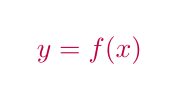
\begin{tikzpicture}
    \axes
    \fctn{purple,very thick}
    \node[purple,below right] at (5,-.5) {$y=f(x)$};
  \end{tikzpicture}
\end{center}
First of all, we can regard $f(x)$ itself as a differential form: one which simply does not use the variable $\dx$ (and thus takes the same value regardless of what $\dx$ is).
Thus, each little piece of the graph of this differential form will be a horizontal line, as shown below (we have included the graph of $f$ for comparison).
\begin{center}
  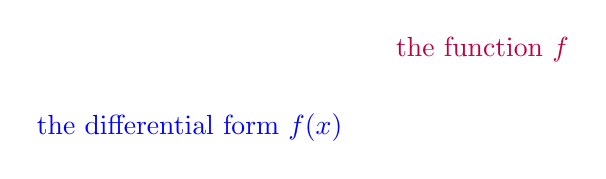
\begin{tikzpicture}
    \axes
    \fctn{dashed,purple}
    \node[purple,right] at (5,-.5) {the function $f$};
    \foreach \x/\y in \heights \draw[blue,very thick] (\x-.3,\y) -- (\x+.3,\y);
    \node[blue] at (2.5,-1.5) {the differential form $f(x)$};
  \end{tikzpicture}
\end{center}
This seems a little odd as a representation of $f$, so we may ask whether there is some differential form for which each piece of its graph looks like a corresponding part of the graph of $f$ itself.
Such a differential form is $f(x+\dx)$, since as $\dx$ varies around zero, $x+\dx$ varies around $x$.
\begin{center}
  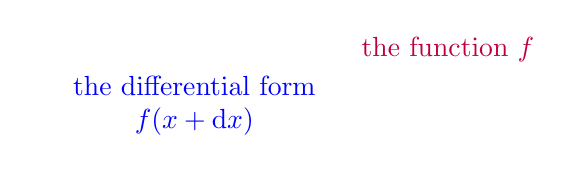
\begin{tikzpicture}
    \axes
    \fctn{dashed,purple}
    \node[purple,below right] at (5,-.5) {the function $f$};
    \foreach \x/\y in \heights {
      \begin{scope}
        \clip (\x-0.3,\y-0.3cm) rectangle (\x+0.3,\y+0.3cm);
        \fctn{blue,very thick}
      \end{scope}
    }
    \node[blue] at (3,-1.5) {\parbox{4cm}{\centering the differential form\\$f(x+\dx)$}};
  \end{tikzpicture}
\end{center}
Finally, consider the differential form $f(x+\dx)-f(x)$.
Its graph at $x$ looks just like a piece of the graph of $f$ near $x$, just as for the form $f(x+\dx)$, but now this graph is shifted down so that it crosses the $x$-axis at the point $(x,0)$ (this is what subtracting $f(x)$ accomplishes).
\begin{center}
  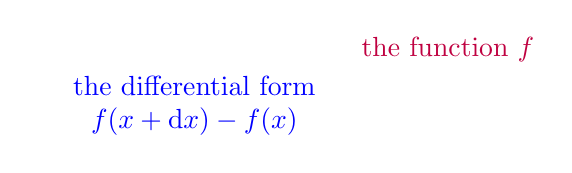
\begin{tikzpicture}
    \axes
    \fctn{dashed,purple}
    \node[purple,below right] at (5,-.5) {the function $f$};
    \foreach \x/\y in \heights {
      \begin{scope}
        \clip (\x-.3,-.3) rectangle (\x+0.3,.3);
        \fctn{blue,very thick,yshift=-\y}
      \end{scope}
    }
    \node[blue] at (3,-1.5) {\parbox{4cm}{\centering the differential form\\$f(x+\dx)-f(x)$}};
  \end{tikzpicture}
\end{center}
Note that the pieces of the graph of $f(x+\dx)-f(x)$ all look quite close to straight lines.
This happens whenever we ``zoom in'' sufficiently on a smooth function, and it is this observation that leads to the idea of differentiation.

\section{Graphing differential forms in more dimensions}
\label{sec:graphing-higher-dim}

TODO.

\section{Differentials}
\label{sec:differentials}

In one-variable calculus, you may have encountered the differential of a function.
Namely, if $f$ is a function of one variable $x$, then its differential is
\begin{equation}
  \df = f'(x) \, \dx\label{eq:onevariable-differential}
\end{equation}
where $f'$ is the \emph{derivative} of $f$.
Note that $\df$ is a differential form.
Its graph looks like this (the function $f$ is the same one we were using as an example at the end of \cref{sec:graphing-differential-forms}).
\begin{center}
  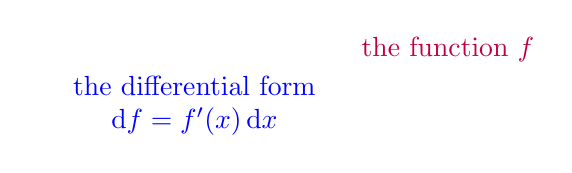
\begin{tikzpicture}
    \axes
    \fctn{dashed,purple}
    \node[purple,below right] at (5,-.5) {the function $f$};
    \foreach \x/\y/\slope in \heights {
      \begin{scope}
        \clip (\x-.3,-.3) rectangle (\x+0.3,.3);
        % \fctn{red,very thick,yshift=-\y}
        \draw[blue,very thick] (\x-.3,-\slope) -- (\x+.3,\slope);
      \end{scope}
    }
    \node[blue] at (3,-1.5) {\parbox{4cm}{\centering the differential form\\$\df = f'(x) \,\dx$}};
  \end{tikzpicture}
\end{center}
Note that this is barely distinguishable from the graph of $f(x+\dx)-f(x)$.
This is the whole point of the derivative: $f'(x)$ is the slope of the tangent line to the graph of $f$ at $x$, and that line is the best possible \emph{linear approximation} to the graph.
Indeed, recall that by definition, the derivative is
\[ f'(x) = \lim_{\dx\to 0} \frac{f(x+\dx)-f(x)}{\dx} \]
Thus, when $\dx$ is small, we can say that
\begin{equation}\label{eq:difference-quotient-close-derivative}
  \frac{f(x+\dx)-f(x)}{\dx}\quad\text{is very close to}\quad f'(x).
\end{equation}
Multiplying each of these by $\dx$, we find that
\begin{equation}
  f(x+\dx)-f(x) \quad\text{is very close to}\quad f'(x)\,\dx.\label{eq:difference-close-differential}
\end{equation}
This is what we saw in the above-remarked similarity of graphs.

\begin{adv}
  However, the quantities in~\cref{eq:difference-close-differential} are of a different order than those in~\cref{eq:difference-quotient-close-derivative}:
  $\frac{f(x+\dx)-f(x)}{\dx}$ and $f'(x)$ are zeroth order, while $f(x+\dx)-f(x)$ and $f'(x)\,\dx$ are first order.
  Thus, the precise meaning of ``close'' is different: in~\cref{eq:difference-close-differential} we mean that their difference is first order, while in~\cref{eq:difference-quotient-close-derivative} we mean that their difference is second order.
  This is why \cref{def:differential} below is phrased as it is.
\end{adv}

\Cref{eq:onevariable-differential} from one-variable calculus defines the \emph{differential} of $f$ in terms of the \emph{derivative} of $f$.
However, in multivariable calculus, it is more appropriate to do things in the other order, using the idea of~\cref{eq:difference-quotient-close-derivative} to define the differential \emph{first}, and then deducing a notion of ``derivative'' from this.

\begin{defn}\label{def:differential}
  If $f$ is a function of a point $\ptx$, then its \textbf{differential} is a linear differential form $\df$ such that
  \[ f(\ptx + \dd\ptx) - f(\ptx) - \df \]
  is negligible at $\ptx$.
  If such a form $\df$ exists, we say that $f$ is \textbf{differentiable} at $\ptx$.
\end{defn}

As always, we should explore a new definition with examples.

\begin{eg}
  Let $f(x) = x^2$, an ordinary one-variable function.
  Then
  \begin{align*}
    f(x + \dx) - f(x) &= (x+\dx)^2 - x^2\\
    &= x^2 + 2 x \, \dx + \dx^2 - x^2\\
    &= 2x \, \dx + \dx ^2.
  \end{align*}
  What linear form $\dd f$ can we subtract from this to make it second order?
  We may think of subtracting $2x \, \dx$, leaving the second-order term $\dx^2$:
  \[ f(x + \dx) - f(x) - 2x \, \dx \;=\; \dx^2. \]
  Thus, we have $\dd(x^2) = 2 x \, \dx$.
  Of course, this is the same result that we would have gotten from \cref{eq:onevariable-differential}.
\end{eg}

\begin{eg}
  Even more simply, let $f(x) = x$.
  Then
  \[f(x+\dx) - f(x) = (x+\dx)-x = \dx \]
  which is already a linear form.
  Thus, $\dd(x) = \dx$, so the notation is consistent.
\end{eg}

\begin{eg}
  Let $f(x,y) = x^2 + 2y^2 - xy$.
  Then
  \begin{align*}
    f(x+\dx,y+\dy) - f(x,y)
    &= (x+\dx)^2 + 2(y+\dy)^2 - (x+\dx)(y+\dy) - x^2 - 2y^2 + xy\\
    &= x^2 + 2 x \, \dx + \dx^2 + 2y^2 + 4y\,\dy + 2\dy^2\\
    & \hspace{2cm} - x^2 - x \, \dy - y \, dx - \dx\, \dy - x^2 - 2y^2 + xy\\
    &= 2x\,\dx + 4y\,\dy - x\,\dy - y\,\dx + \dx^2 + 2\dy^2 - \dx\,\dy\\
    &= (2x-y)\,\,dx + (4y-x)\,\dy + (\dx^2 + 2\dy^2 - \dx\,\dy)
  \end{align*}
  In the last line we have separated this into a linear form plus one of second order.
  Thus, we have
  \[ \dd(x^2 + 2y^2 - xy) = (2x-y)\,\dx + (4y-x)\,\dy .\]
\end{eg}

\begin{eg}
  Consider $f(x) = \sin x$.
  Using the sum identity for sine, we have
  \begin{align}
    \sin(x+\dx) - \sin (x)
    &= \sin x \cos \dx + \sin \dx \cos x - \sin x \notag\\
    &= \cos x \sin \dx + (\sin x) (\cos \dx - 1).\label{eq:sine-difference}
  \end{align}
  The usual way to proceed from here is to recall the limits
  \[ \lim_{h\to 0} \frac{\sin h}{h} = 1 \qquad\text{and}\qquad
  \lim_{h\to 0} \frac{\cos h - 1}{h} = 0 \]
  The second says exactly that the form $\cos \dx - 1$ is negligible.
  The first one implies that
  \[ \lim_{\dx\to 0} \frac{\sin \dx - \dx}{\dx} = 0 \]
  and therefore the form $\sin \dx - \dx$ is negligible.
  Multiplying by the ordinary functions $\cos x$ and $\sin x$ doesn't change the order, so we can write
  \begin{align*}
    \sin(x+\dx) - \sin (x)
    &= \cos x \sin \dx + (\sin x) (\cos \dx - 1)\\
    &= (\cos x )(\dx  + \sin \dx - \dx) + (\sin x) (\cos \dx - 1)\\
    &= \cos x \,\dx + (\cos x) (\sin \dx - \dx) + (\sin x) (\cos \dx - 1)
  \end{align*}
  which is written as the linear form $\cos x \,\dx$ plus a negligible one.
  Thus, $\dd(\sin x) = \cos x \,\dx$.

  Another, perhaps more intuitive, way to proceed from \cref{eq:sine-difference} is to recall the power series expansions
  \begin{align*}
    \sin x &= x - \frac{x^3}{3!} + \frac{x^5}{5!} - \cdots\\[2pt]
    \cos x &= 1 - \frac{x^2}{2!} + \frac{x^4}{4!} - \cdots
  \end{align*}
  Therefore, we have
  \begin{align*}
    \sin \dx - \dx &= - \frac{\dx^3}{3!} + \frac{\dx^5}{5!} - \cdots\\[2pt]
    \cos \dx - 1 &= - \frac{\dx^2}{2!} + \frac{\dx^4}{4!} - \cdots.
  \end{align*}
  Using general facts about functions defined by power series, one can conclude from this that the first is third order and the second is second order; thus both are negligible.
  (However, when calculating the power series expansions of sine and cosine in one-variable calculus, you probably used the fact that you already knew their derivatives, so this would technically be a circular argument.)
\end{eg}

A convenient way to work with differentials is to introduce the notion of ``approximation to first order''.

\begin{defn}
  We say that two differential forms $\omega$ and $\eta$ are \textbf{equal to first order} if their difference $\omega-\eta$ is negligible.
  In this case we write
  \[\omega\apx1 \eta.\]
\end{defn}

\begin{eg}
  We have $x\,\dx + \dx^2 \apx1 x\,\dx - e^x \,\dx^2$, since their difference is
  \[ (x\,\dx + \dx^2) - (x\,\dx - e^x\, \dx^2) = (1+e^x)\dx^2 \]
  which is second order.
\end{eg}

The relation $\apx{1}$ behaves roughly like equality.
For instance, we can add or subtract the same differential form from both sides.
In particular, if $\omega$ is negligible, then $\omega\apx{1}0$, so we have $\eta + \omega \apx{1} \eta$ for any $\eta$.

\begin{eg}
  Since $4\,\dx^2$ is second order, we have $\sin(x) \,\dx + 4\, \dx^2 \apx{1} \sin(x)\,\dx$.
\end{eg}

We can also multiply both sides by any differential form that is bounded near $\dx=0$, since multiplying by such a form doesn't affect negligibility.

\begin{eg}
  Since $\sqrt{x}\, \dx^2$ is second order, we have
  \[x\,\dx \apx{1} x\,\dx + \sqrt{x}\, \dx^2\]
  Thus, we can multiply by $e^x$ to get
  \[x e^x \,\dx \apx{1} x e^x\,\dx + \sqrt{x}\, e^x\, \dx^2,\]
  or multiply by $\dx$ to get
  \[x\,\dx^2 \apx{1} x\,\dx^2 + \sqrt{x} \,\dx^3. \]
  The latter is fairly trivial, though since both sides are $\apx{1} 0$.
\end{eg}

Now we can equivalently state the definition of a differential: $\df$ is a linear differential form such that
\[ f(x+\dx) \apx1 f(x) + \df, \]
if such exists.
Our previous calculations of differentials can all be written in this way.
For instance,
\begin{align*}
  (x+\dx)^2 &= x^2 + 2 x\,\dx + \dx^2\\
  &\apx1 x^2 + 2 x\,\dx
\end{align*}
since $\dx^2$ is second order.
Therefore, $\dd(x^2) = 2x\,\dx$.

% TODO: Tangent planes and linear approximations

\section{Differential rules}
\label{sec:differential-rules}

We easily deduce all the usual derivative rules, written in terms of differentials.
For instance, given functions $f$ and $g$, consider their sum $f+g$.
\begin{align*}
  f(x+\dx) + g(x+\dx)
  &\apx1 f(x) + \df + g(x) + \dg\\
  &= \big[f(x) + g(x)\big] + \big[ \df + \df \big]
\end{align*}
Thus, we have
\[ \dd(f+g) = \df + \dg. \]

Similarly, for the product rule, we compute
\begin{align*}
  f(x+\dx) \, g(x+\dx)
  &\apx1 \big(f(x)+\df\big)\big(g(x) + \dg \big)\\
  &= f(x) g(x) + f(x) \,\dg + g(x) \,\df + \df\,\dg\\
  &\apx1 f(x) g(x) + f(x) \,\dg + g(x) \,\df
\end{align*}
since $\df\,\dg$ is a product of two first-order forms, hence second order.
Thus,
\[ \dd(f\,g) = f\,\dg + g\,\df.\]

Importantly, these rules, stated in exactly the same way, apply to functions of more than one variable.
\begin{eg}\label{eg:twovar-differential}
  If $f(x,y) = x^2y + xy^2$, then we can use the sum and product rules to obtain
  \begin{align*}
    \dd(x^2y + xy^2) &= \dd(x^2y) + \dd(xy^2)\\
    &= x^2\,\dy + y \,\dd(x^2) + x \,\dd(y^2) + y^2\,\dx\\
    &= x^2\,\dy + y \,(2x\,\dx) + x\, (2y\,\dy) + y^2\,\dx\\
    &= (2xy + y^2)\,\dx + (x^2+2xy)\,\dy
  \end{align*}
\end{eg}

Finally, the chain rule for differentials is easy to \emph{use}, but tricky to \emph{state}, because the notation makes it look like a triviality.
Suppose that we have a function $f$ of two variables $u$ and $v$, and that $u$ and $v$ are each themselves functions of two other variables $x$ and $y$.
Then the statement of the chain rule is that if we calculate $\df$ treating $u$ and $v$ as its input variables (obtaining a linear differential form involving $\du$ and $\dv$), and likewise we calculate the differentials $\du$ and $\dv$ treating $x$ and $y$ as their input variables (obtaining linear differential forms involving $\dx$ and $\dy$), then substitute the latter into the former, as well as the values of $u$ and $v$ in terms of $x$ and $y$, we obtain the same expression for $\df$ in terms of $\dx$ and $\dy$ that we would have if we first substituted the functions $u$ and $v$ and then took the differential treating $x$ and $y$ as the input variables.

If you found that totally incomprehensible, you're in good company; I barely understood it as I was writing it.
It is much better explained by an example.

\begin{eg}
  Let $f(u,v) = u v + 3u$, while $u(x,y) = x-5y$ and $v(x,y) = 4y-x$.
  Then
  \begin{align*}
    \df &= \dd(u v) + \dd(3u)\\
    &= v \,\du + u\,\dv + 3 \,\du\\
    &= (v+3)\,\du + u\,\dv
  \end{align*}
  and
  \begin{align*}
    \du &= \dx - 5\, \dy\\
    \dv &= 4\,\dy - \dx
  \end{align*}
  Therefore,
  \begin{align*}
    \df &= (v+3)\,\du + u\,\dv\\
    &= (4y-x+3)\,(\dx - 5 \dy) + (x-5y) (4\,\dy - \dx) \\
    &= (9y-2x+3)\,\dx + (9x - 40y - 15)\,\dy.
  \end{align*}
  On the other hand, if we substituted first, we would have
  \begin{align*}
    f(u(x,y),v(x,y)) &= (x-5y)(4y-x) + 3(x-5y)\\
    &= 4xy - x^2 - 20y^2 + 5xy + 3x - 15 y\\
    &= 9xy - x^2 - 20y^2 + 3x - 15 y
  \end{align*}
  and therefore
  \begin{align*}
    \df &= 9x\, \dy + 9y\, \dx - 2 x\,\dx - 40 y\,\dy + 3\,\dx - 15\,\dy\\
    &= (9y - 2x +3)\,\dx + (9x - 40y - 15)\,\dy
  \end{align*}
  which is the same result.
\end{eg}

Thus, the chain rule for differentials basically says that differentials obey the usual rules of algebra: if a differential $\du$ is equal to some other differential form, then we can substitute the latter for the former.
It's important to note that even though it looks obvious, this \emph{is} a nontrivial \emph{theorem} that requires proof, although we will not prove it.
\begin{notextbook}(It might be proven in your textbook.)\end{notextbook}

When expressed in terms of differentials in this way, the chain rule is also known as \emph{Cauchy's invariant rule}.
Of course, it is mainly useful in cases where we are given the result of substitution, but where it is not obvious how to find the differential until we decompose it.

\begin{eg}
  Consider the function $f(x,y) = \sin (xy)$.
  We can find the differential by letting $u=xy$; then we have $f = \sin(u)$, and hence
  \begin{align*}
    \df &= \cos(u)\,\du\\
    \du &= x\,\dy + y\,\dx
  \end{align*}
  and therefore
  \begin{align*}
    \df &= \cos(u)\,\du \\
    &= \cos(xy) (x\,\dy + y\,\dx)\\
    &= y\cos(xy)\,\dx + x\cos(xy)\,\dy
  \end{align*}
  Once we are more familiar with the operation of the chain rule, this calculation can be done without naming the variable $u$.
  We simply remember that in the rule for the derivative of the sine function, $\dd(\sin(x)) = \cos(x) \, \dx$, the variable $x$ can be replaced by \emph{any expression}, as long as we also remember to replace $\dx$ by the differential of \emph{that expression}.
  \begin{align*}
    \df &= \dd(\sin(xy))\\
    &= \cos(xy) \, \dd(xy)\\
    &= \cos(xy) (x\,\dy + y\,\dx)\\
    &= y\cos(xy)\,\dx + x\cos(xy)\,\dy.
  \end{align*}
\end{eg}

A particularly important example of the chain rule is translating between different coordinate systems.
Recall that in addition to the usual ``rectangular'' or ``Cartesian'' coordinates $x$ and $y$ on the plane, we can use \emph{polar coordinates} $r$ and $\theta$, which are related by the equations
\begin{alignat*}{2}
  x &= r \cos \theta &\qquad r &= \sqrt{x^2+y^2}\\
  y &= r \sin\theta &\qquad \tan \theta &= y/x
\end{alignat*}
(It would not be correct to write ``$\theta = \arctan(y/x)$'', since $\arctan$ only takes values between $-\pi/2$ and $\pi/2$, whereas $\theta$ usually ranges from $0$ to $2\pi$.)
Differentiating these equations, we obtain corresponding equations relating the differentials of these variables.
\begin{align}
  \dx &= \cos \theta \,\dr - r \sin\theta \,\dtheta \label{eq:polar-dx} \\
  \dy &= \sin\theta \,\dr + r \cos\theta\,\dtheta \label{eq:polar-dy}\\
  \dr &= \frac{1}{2\sqrt{x^2+y^2}}(2x\,\dx + 2y\,\dy) \notag\\
  &= \frac{x}{\sqrt{x^2+y^2}}\,\dx + \frac{y}{\sqrt{x^2+y^2}}\,\dy
  \qquad\left(= \frac{x}{r} \,\dx + \frac{y}{r}\,\dy\right) \notag\\
  \frac{1}{(\cos \theta)^2} \,\dtheta &= \frac{1}{x}\,\dy - \frac{y}{x^2}\,\dx \notag\\
  \dtheta &= (\cos \theta)^2 \left( \frac{r}{r^2\cos\theta}\,\dy - \frac{y}{r^2 (\cos\theta)^2}\,\dx\right) \notag\\
  &= \frac{x}{r^2} \,\dy - \frac{y}{r^2} \,\dx \notag\\
  &= \frac{x}{x^2+y^2} \,\dy - \frac{y}{x^2+y^2} \,\dx \notag
\end{align}
(We could also obtain the same equations for $\dr$ and $\dtheta$ by solving for them in the first two equations.)
It follows that if $f$ is written as a function of $x$ and $y$, we can find its differential with respect to $r$ and $\theta$ by substituting these relations into its differential with respect to $x$ and $y$, and vice versa.

\begin{eg}
  Suppose $f(x,y) = e^{x^2+y^2}$.
  Then we have
  \begin{align*}
    \df &= e^{x^2+y^2} (2x \,\dx + 2y\,\dy)\\
    &= 2x e^{x^2+y^2} \,\dx + 2y e^{x^2+y^2} \,\dy\\
    &= 2 r\cos\theta e^{r^2} \, (\cos \theta \,\dr - r \sin\theta \,\dtheta) + 2r\sin\theta e^{r^2} (\sin\theta \,\dr + r \cos\theta\,\dtheta)\\
    &= 2r e^{r^2} ((\cos\theta)^2 + (\sin\theta)^2)\,\dr + 2r^2 e^{r^2}(\sin\theta\cos\theta - \cos\theta\sin\theta) \dtheta\\
    &= 2r e^{r^2}\,\dr.
  \end{align*}
  which is the same result that we could calculate directly by writing $f = e^{r^2}$ and thus
  \begin{align*}
    \df &= e^{r^2} \, (2r\,\dr).
  \end{align*}
\end{eg}

Similarly, in three-dimensional space, in addition to the rectangular coordinates $x$, $y$, and $z$, we have both \emph{cylindrical} coordinates $r$, $\theta$, and $z$, and \emph{spherical} coordinates $\rho$, $\theta$, and $\phi$.
Cylindrical coordinates are related to rectangular ones in three dimensions in the same way that polar coordinates are related to rectangular ones in two dimensions, with $z$ coming along untouched for the ride.
For spherical coordinates we have
\begin{align*}
  x &= \rho \cos\theta \sin\phi\\
  y &= \rho \sin\theta \sin\phi\\
  z &= \rho\cos\phi
\end{align*}
and hence
\begin{align*}
  \dx &= \cos\theta \sin\phi \,\drho - \rho\sin\theta\sin\phi \,\dtheta + \rho\cos\theta\cos\phi \,\dphi\\
  \dy &= \sin\theta \sin\phi\,\drho + \rho\cos\theta\sin\phi \,\dtheta + \rho\sin\theta\cos\phi \,\dphi\\
  \dz &= \cos\phi\,\drho - \rho\sin\phi\,\dphi
\end{align*}
We leave it to the reader to write out the reverse expressions for spherical coordinates in terms of rectangular ones.


\section{Derivatives}
\label{sec:derivatives}

We can now define the \emph{derivative} in terms of the \emph{differential}.
Note that in one dimension, a linear differential form must be of the form
\[ g(x) \,\dx \]
for some function $g$.
In particular, if $f$ is a differentiable function of one variable $x$, then since its differential $\df$ is by definition a \emph{linear} differential form, we must have $\df = g(x) \, \dx$ for some function $g$.
We call the function $g$ the \emph{derivative} of $f$ and denote it by $f'$.
In other words, we have
\[\df = f'(x)\,\dx\]
(which is \cref{eq:onevariable-differential}), or
\[ f'(x) = \frac{\df}{\dx}. \]
This is a notation for the derivative that you have probably seen before.
The point is that now, we have given separate meanings to $\dx$ and $\df$, and \emph{defined} $f'(x)$ to be their quotient.

However, when there is more than one variable, this doesn't work any more!
For instance, consider the function $f(x,y) = x^2y + xy^2$, whose differential we found in \cref{eg:twovar-differential} to be
\[ \df = (2xy + y^2)\,\dx + (x^2+2xy)\,\dy.\]
Since there are two variables $x$ and $y$, there are two differentials $\dx$ and $\dy$ appearing in this expression for $\df$.
Thus, we can no longer simply divide $\df$ by $\dx$ to get a simple function.
We could of course write
\begin{align*}
  \frac{\df}{\dx} &= (2xy + y^2) + (x^2+2xy)\frac{\dy}{\dx} \qquad\text{or}\\[2pt]
  \frac{\df}{\dy} &= (2xy + y^2)\frac{\dx}{\dy} + (x^2+2xy)
\end{align*}
but in neither case is the right-hand side an ordinary function of $x$ and $y$.
We conclude that\\
\begin{center}
  \fbox{\emph{It makes no sense to talk of ``the'' derivative of a function of more than one variable!}}
\end{center}
\vspace{5mm}
However, we do have two ordinary functions that have about an equal claim to be called a ``derivative'' of our function $f$ above, namely $2xy + y^2$ and $x^2+2xy$.
Neither one ``tells the whole story'' about the differential $\df$ on its own, but together they do.
Thus, we refer to each of them as a \emph{partial derivative} of $f$.

\begin{defn}
  If $f$ is a differentiable function of two variables $x,y$, then its \textbf{partial derivatives} are the functions $\pder{f}{x}$ and $\pder{f}{y}$ such that
  \[ \df = \pder{f}{x}\,\dx + \pder{f}{y}\,\dy\]
  Similarly, if $f$ is a differentiable function of three variables $x,y,z$, then its partial derivatives $\pder{f}{x}$, $\pder{f}{y}$, and $\pder{f}{z}$ are the functions such that
  \[ \df = \pder{f}{x}\,\dx + \pder{f}{y}\,\dy + \pder{f}{z}\,\dz.\]
\end{defn}

The symbol $\partial$ is a stylized ``$d$'' and is pronounced either ``del'' or ``partial''.
Note that unlike for ordinary one-variable derivatives, the symbols $\partial f$ and $\partial x$ have \emph{no meaning} on their own.

\begin{eg}
  For the function $f(x,y) = x^2y + xy^2$ with $\df = (2xy + y^2)\,\dx + (x^2+2xy)\,\dy$, we have
  \begin{align*}
    \pder{f}{x} = 2xy + y^2 \qquad\text{and}\qquad
    \pder{f}{y} = x^2+2xy.
  \end{align*}
\end{eg}

There are many other notations for partial derivatives: $\pder{f}{x}$ may also be written as $f_x$, $\partial_x f$, $D_x f$, or $D_1 f$.

Now recall that a differential form is, formally, a function on vectors, with $\dx$ and $\dy$ representing the components of the input vector.
The partial derivatives (in two dimensions) can then equivalently be defined by \emph{evaluating} this function at the unit vectors $\vcc{1,0}$ and $\vcc{0,1}$:
\begin{align*}
  \df(\ptx,\vcc{1,0}) &= \pder{f}{x}\cdot 1 + \pder{f}{y}\cdot 0 = \pder{f}{x}\\[2pt]
  \df(\ptx,\vcc{0,1}) &= \pder{f}{x}\cdot 0 + \pder{f}{y}\cdot 1 = \pder{f}{y}.
\end{align*}
(Similarly, in three dimensions we evaluate at the three unit vectors.)
More generally, the result of evaluating $\df$ at $\vc{v}$ is called the \textbf{directional derivative} of $f$ along a vector $\vc{v}$.
It has the following interpretation as a one-variable derivative.

\begin{thm}
  Given a point $\ptx$ and a vector $\vc{v}$ based at $\ptx$, define a function $g_{\vc{v}}$ by
  \[ g_{\vc{v}}(t) = f(\ptx + t \vc{v}). \]
  Then the directional derivative of $f$ along $\vc{v}$ is equal to the derivative of $g_{\vc{v}}$ at $0$:
  \[ \df(\ptx,\vc{v}) = g_{\vc{v}}'(0). \]
\end{thm}

In particular, when $\vc{v}$ is $\vcc{1,0}$ or $\vcc{0,1}$, we obtain the following expressions for the partial derivatives (in two dimensions):
\begin{alignat*}{2}
  \pder{f}{x} &= g_{\vcc{1,0}}'(0) \qquad\text{where}\qquad & g_{\vcc{1,0}}(t) &= f(x+t,y)\\[2pt]
  \pder{f}{x} &= g_{\vcc{0,1}}'(0) \qquad\text{where}\qquad & g_{\vcc{0,1}}(t) &= f(x,y+t).
\end{alignat*}
This means that $\pder{f}{x}$ can also be interpreted as \emph{the derivative of $f$ with respect to $x$, with $y$ treated as a constant}, and similarly for $\pder{f}{y}$.

We may also speak of directional derivatives and partial derivatives of a function that is not known to be differentiable.
In this case we \emph{define} them by the above formulas.
If we expand out the definition of the derivative, this becomes:
\begin{align}
  \pder{f}{x} &= \lim_{t\to 0} \frac{f(x+t,y) - f(x,y)}{t}\\[2pt]
  \pder{f}{x} &= \lim_{t\to 0} \frac{f(x,y+t) - f(x,y)}{t}.
\end{align}
\begin{notextbook}Your textbook should contain further discussion of partial derivatives and directional derivatives.\end{notextbook}%
\begin{stewart}The textbook takes this approach in Chapter 11, defining partial derivatives first in section 11.3, and then the differential (or ``total differential'') in section 11.4.\end{stewart}

One thing in particular that is worth noting is how the chain rule manifests itself in terms of partial derivatives.
If $f$ is a function of $u$ and $v$, with $u$ and $v$ each functions of $x$ and $y$, then we have
\begin{align*}
  \df &= \pder{f}{u}\,\du + \pder{f}{v}\,\dv\\
  &= \pder{f}{u}\,\left(\pder{u}{x}\,\dx + \pder{u}{y}\,\dy\right) + \pder{f}{v}\,\left(\pder{v}{x}\,\dx + \pder{v}{y}\,\dy\right)\\
  &= \left(\pder{f}{u}\pder{u}{x}+ \pder{f}{v}\pder{v}{x}\right)\dx + \left(\pder{f}{u}\pder{u}{y}+ \pder{f}{v}\pder{v}{y}\right)\dy.
\end{align*}
Since we also have
\[ \df = \pder{f}{x}\,\dx + \pder{f}{y}\,\dy \]
it must be the case that
\begin{equation}\label{eq:partial-chain-rule}
  \pder{f}{x} = \pder{f}{u}\pder{u}{x}+ \pder{f}{v}\pder{v}{x}
  \qquad\text{and}\qquad
  \pder{f}{y} = \pder{f}{u}\pder{u}{y}+ \pder{f}{v}\pder{v}{y}.
\end{equation}
In other words, the chain rule for a partial derivative $\pder{f}{x}$ has one term for each intermediate function $u$ and $v$, each of which looks like the usual chain rule but with partial derivatives instead of ordinary ones.
\begin{stewart}This is the only form of the multivariable chain rule that is discussed in the textbook (section 11.5).\end{stewart}

For instance, note that \cref{eq:polar-dx,eq:polar-dy} yield the partial derivatives
\begin{alignat*}{2}
  \pder{x}{r} &= \cos\theta &\qquad
  \pder{x}{\theta} &= -r\sin\theta\\[3pt]
  \pder{y}{r} &= \sin\theta &\quad
  \pder{y}{\theta} &= r\cos\theta.
\end{alignat*}
Thus, for any function $f$, we have
\begin{align*}
  \pder{f}{r} % &= \pder{f}{x}\pder{x}{r}+ \pder{f}{y}\pder{y}{r}\\
  &= \pder{f}{x} \cos\theta + \pder{f}{y} \sin\theta\\[3pt]
  \pder{f}{\theta} % &= \pder{f}{x}\pder{x}{\theta}+ \pder{f}{y}\pder{y}{\theta}\\
  &= -\pder{f}{x} r\sin\theta + \pder{f}{y} r \cos \theta.
\end{align*}
In practice, is often easier to apply the chain rule by calculating the differentials and substituting, rather than remembering \cref{eq:partial-chain-rule}.


\section{Differential forms versus vectors}
\label{sec:forms-vs-vectors}

Let $\vc{v}$ be a \emph{vector field}, i.e.\ a function assigning to each point $\ptx$ a vector $\vc{v}(\ptx)$ based at $\ptx$.
Such a field is determined by one coordinate function for each dimension.
For example, in three dimensions, we can write
\[ \vc{v}(\ptx) = \vcc{f(\ptx),g(\ptx),h(\ptx)} \]
for some functions $f$, $g$, and $h$ of three variables.

Given such a vector field $\vc{v}$, there is a canonical linear differential form, defined by taking the dot product of $\vc{v}(\ptx)$ with $\dpx$:
\[ \dotp{\vc{v}(\ptx)}{\dpx} = f(\ptx)\,\dx + g(\ptx)\,\dy + h(\ptx)\,\dz. \]
Moreover, any \emph{linear} differential form arises in this way.
For by definition, a form is linear if it can be written as $f(\ptx)\,\dx + g(\ptx)\,\dy + h(\ptx)\,\dz$; and this is equal to $\dotp{\vc{v}(\ptx)}{\dpx}$ if we define $\vc{v}(\ptx) = \vcc{f(\ptx),g(\ptx),h(\ptx)}$.
If $\omega$ is a linear differential form, we call the corresponding vector field its \emph{transpose}.

\begin{defn}
  If $\omega(\ptx,\dpx) = f(\ptx)\,\dx + g(\ptx)\,\dy + h(\ptx)\,\dz$ is a linear differential form, we write $\tr{\omega}$ for its \textbf{transpose}, which is the vector field with the same components:
  \[ \tr{\omega}(\ptx) = \vcc{f(\ptx), g(\ptx), h(\ptx)}. \]
  The definition in two dimensions is analogous.
\end{defn}

Thus by definition we have
\begin{equation}\label{eq:dot-transpose}
  \omega = \dotp{\tr{\omega}}{\dpx}.
\end{equation}

The transpose of the differential of a function has a special name: it's called the \textbf{gradient} of the function, and written $\grad f$.
That is,
\begin{align*}
  \grad f &= \ptr{\df}\\
  &= \lrvcc{\pder{f}{x},\,\pder{f}{y},\,\pder{f}{z}} \qquad\text{(in three dimensions)}
\end{align*}
For the gradient, \cref{eq:dot-transpose} becomes
\[ \df = \dotp{\grad f}{\dpx}. \]
This explains why in vector calculus one often sees dot products with the gradient.
What is really going on is just evaluating the differential.

Part of the importance of the gradient is that it points in the direction of ``steepest increase'' of the function.
More precisely, the directional derivative $\df(\ptx,\vc{v})$ is greatest (for $\vc{v}$ of unit length) when $\vc{v}$ points in the direction of $\grad f(\ptx)$.
\begin{notextbook}More about the gradient can probably be found in your textbook.\end{notextbook}%
\begin{stewart}The textbook discusses gradients in section 11.6.\end{stewart}


\end{document}
